\section{Triggers}

\def\figpath{figures/nr-int-note/trigger/V1/}

\begin{equation}
\text{Multi \Pqb-jet trigger SF} =  \textcolor{hdbs:outrageousorange}{\prod_i SF_{jet}^{kinematic}(i)} \times \textcolor{hh:medturquoise}{ \prod_j SF_{jet}^{b-tag}}
 \end{equation}

\begin{itemize}

\item  \textcolor{hdbs:outrageousorange}{ Kinematic SFs derived in dedicated $t\bar{t}$ analysis}
\item \textcolor{hdbs:outrageousorange}{ Product taken over jets (sorted by \pT) until encountering the 4 HC jets}
\item \textcolor{hh:medturquoise}{ \Pqb-jet trigger SFs provided by the \Pqb-jet trigger group (although they were customly rederived down to 30 GeV since we were investigating a low \pT category).
}
\end{itemize}

\textcolor{red}{I need to revise the RR code, because I think that we actually are looking at \emph{all} of the jets in the event.}

\hl{I really don't think that I want this whole figure, but I am leaving it as a placeholder until I decide how to widdle it down.}
\begin{figure}[]
        \centering
        \subfloat[SM ggF \kl=1]{
                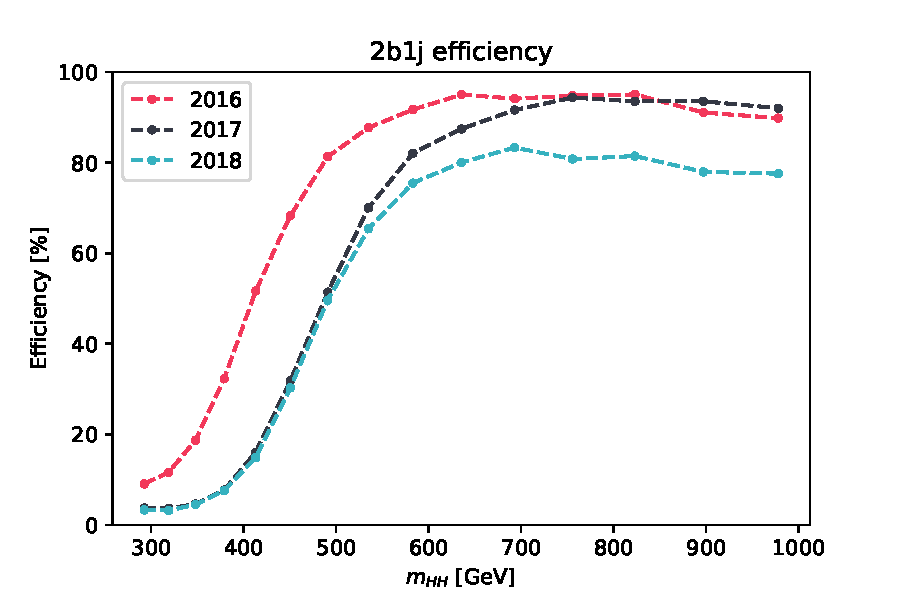
\includegraphics[width=0.33\textwidth]{\figpath/SMNR_ggF_600043-2b1j-trigger-efficiency.pdf}
                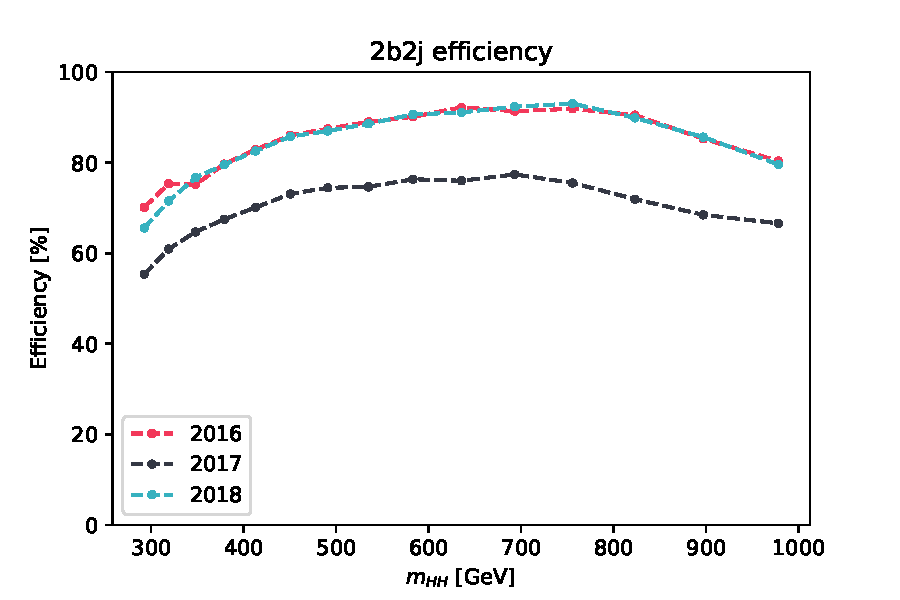
\includegraphics[width=0.33\textwidth]{\figpath/SMNR_ggF_600043-2b2j-trigger-efficiency.pdf}
                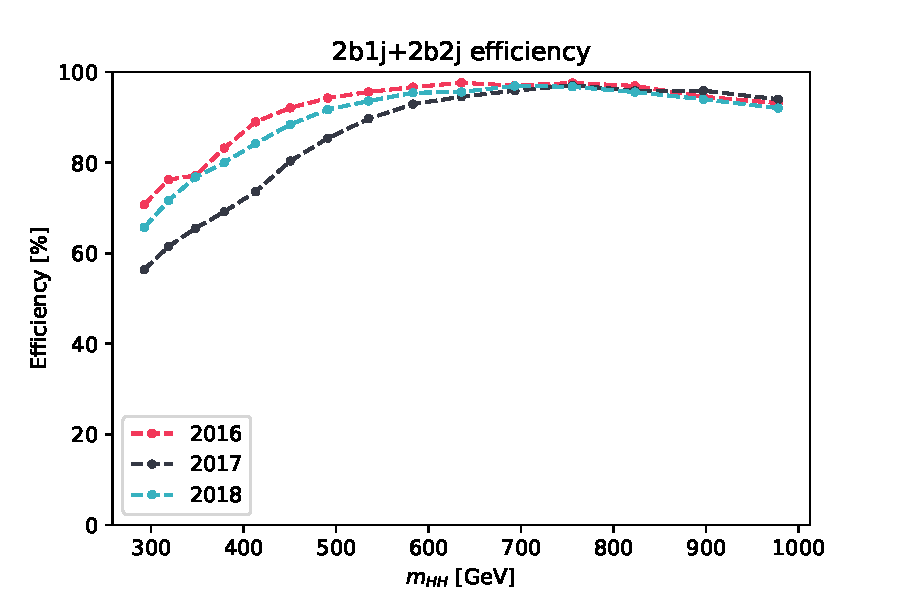
\includegraphics[width=0.33\textwidth]{\figpath/SMNR_ggF_600043-2b1j+2b2j-trigger-efficiency.pdf}
        }\\
        \subfloat[ggF \kl=10]{
                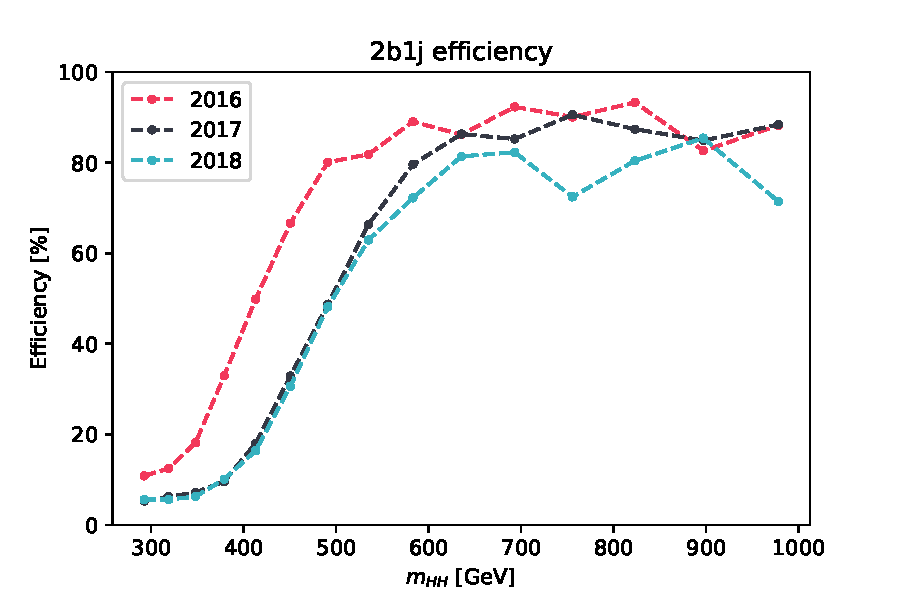
\includegraphics[width=0.33\textwidth]{\figpath/SMNR_ggF_600044-2b1j-trigger-efficiency.pdf}
                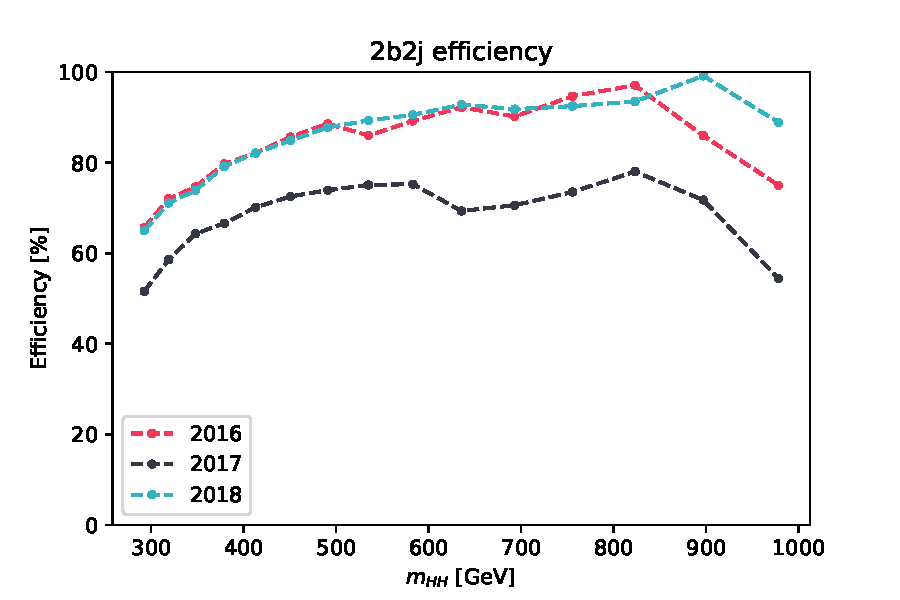
\includegraphics[width=0.33\textwidth]{\figpath/SMNR_ggF_600044-2b2j-trigger-efficiency.pdf}
                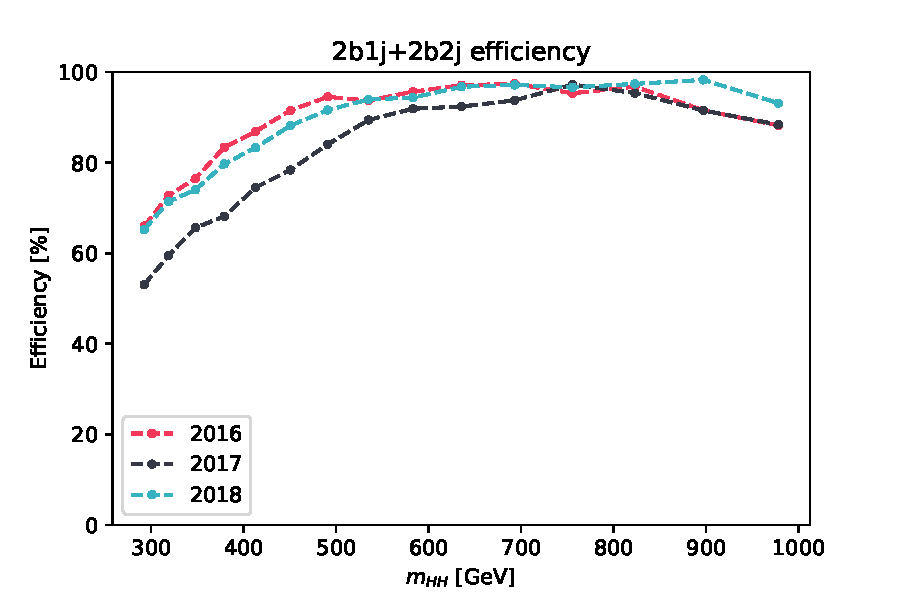
\includegraphics[width=0.33\textwidth]{\figpath/SMNR_ggF_600044-2b1j+2b2j-trigger-efficiency.pdf}
        }\\
        \subfloat[SM VBF \kl=1, \kvv=1]{
                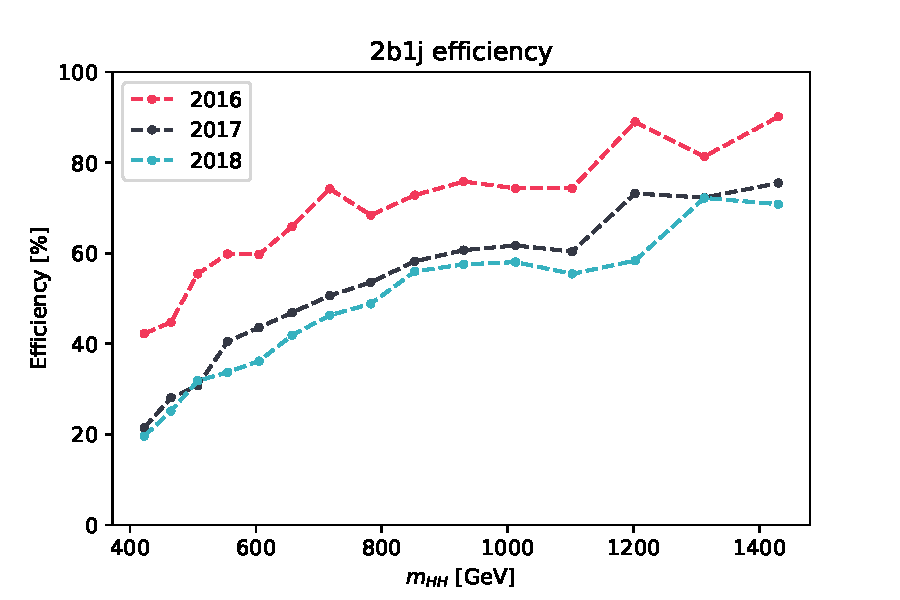
\includegraphics[width=0.33\textwidth]{\figpath/SMNR_VBF_502970-2b1j-trigger-efficiency.pdf}
                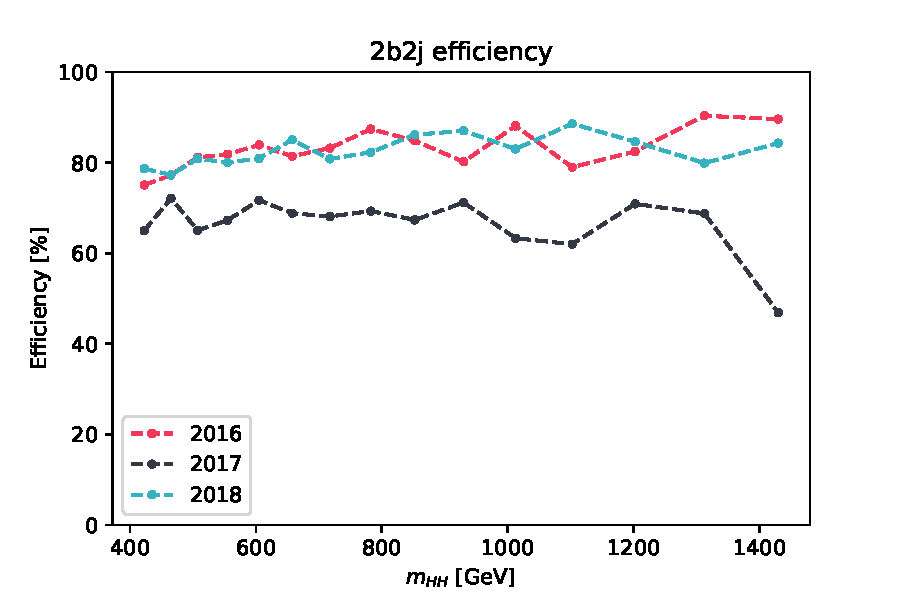
\includegraphics[width=0.33\textwidth]{\figpath/SMNR_VBF_502970-2b2j-trigger-efficiency.pdf}
                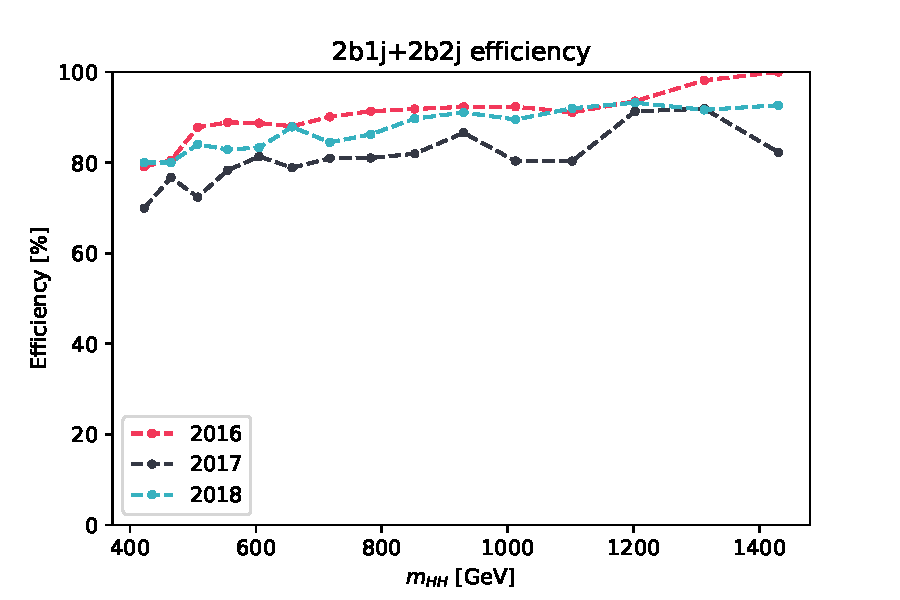
\includegraphics[width=0.33\textwidth]{\figpath/SMNR_VBF_502970-2b1j+2b2j-trigger-efficiency.pdf}
        }\\
        \subfloat[VBF \kl=1, \kvv=0]{
                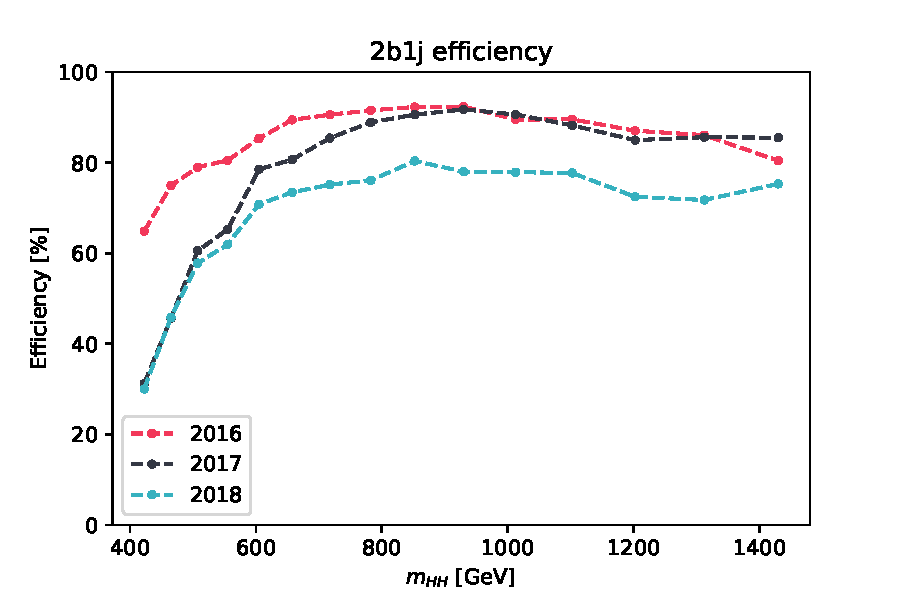
\includegraphics[width=0.33\textwidth]{\figpath/SMNR_VBF_502971-2b1j-trigger-efficiency.pdf}
                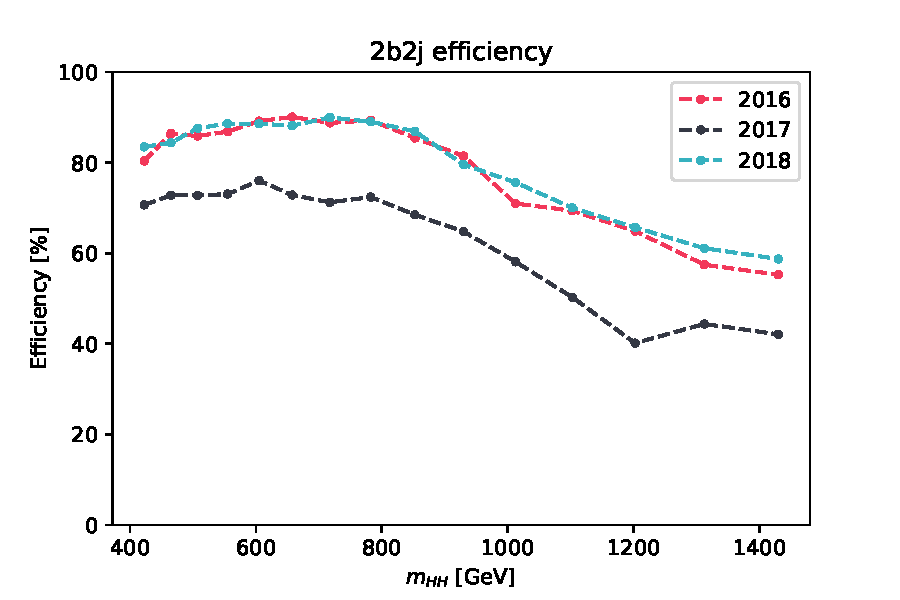
\includegraphics[width=0.33\textwidth]{\figpath/SMNR_VBF_502971-2b2j-trigger-efficiency.pdf}
                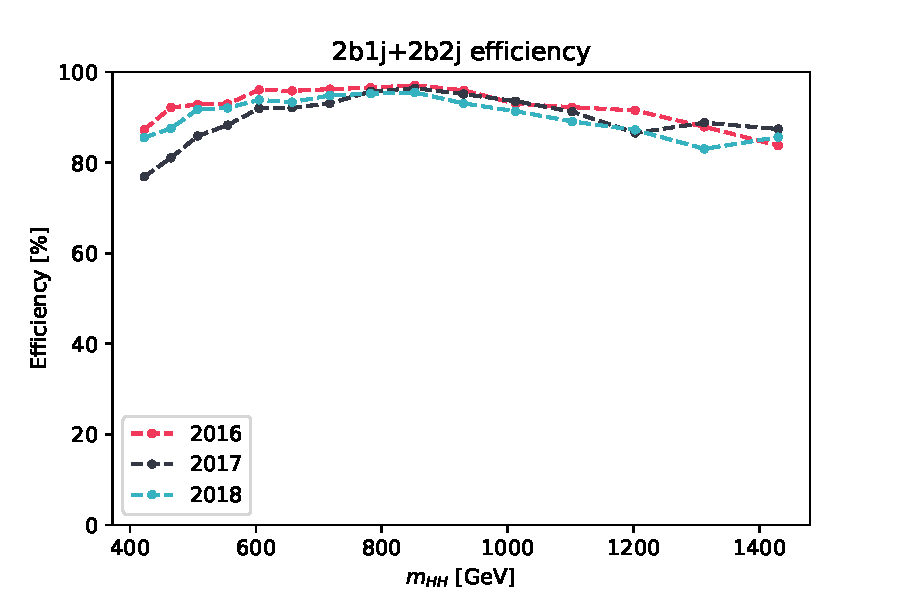
\includegraphics[width=0.33\textwidth]{\figpath/SMNR_VBF_502971-2b1j+2b2j-trigger-efficiency.pdf}
        }\\
        \subfloat[VBF \kl=10, \kvv=1]{
                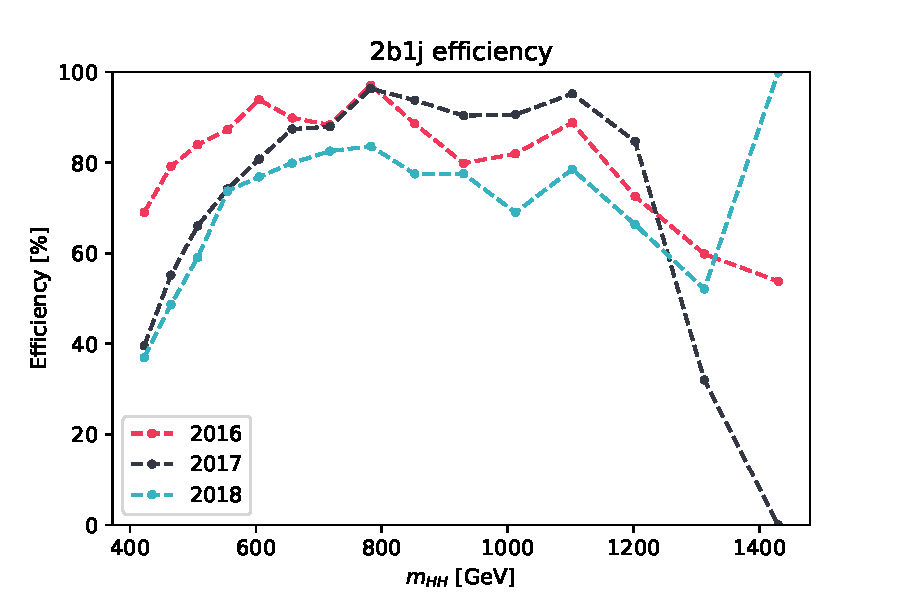
\includegraphics[width=0.33\textwidth]{\figpath/SMNR_VBF_502978-2b1j-trigger-efficiency.pdf}
                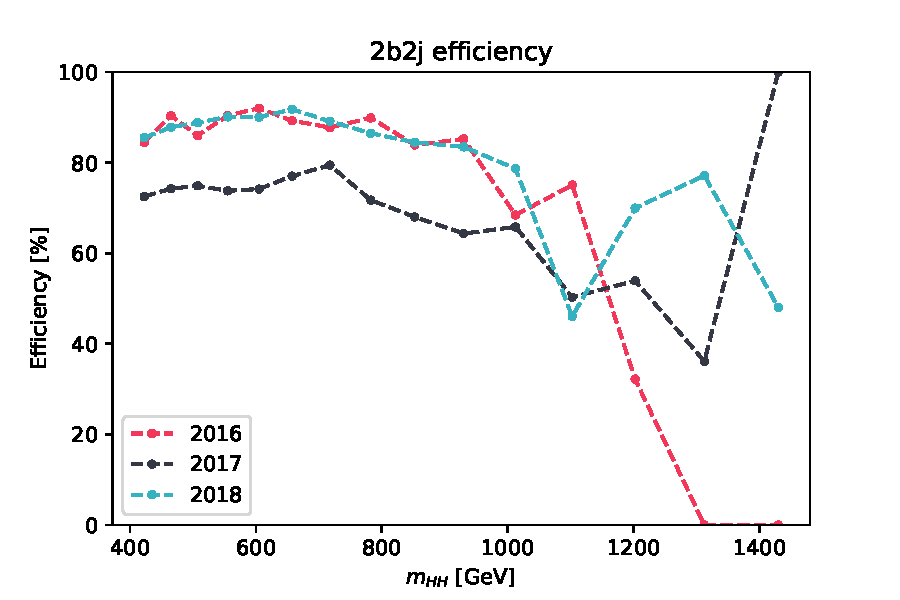
\includegraphics[width=0.33\textwidth]{\figpath/SMNR_VBF_502978-2b2j-trigger-efficiency.pdf}
                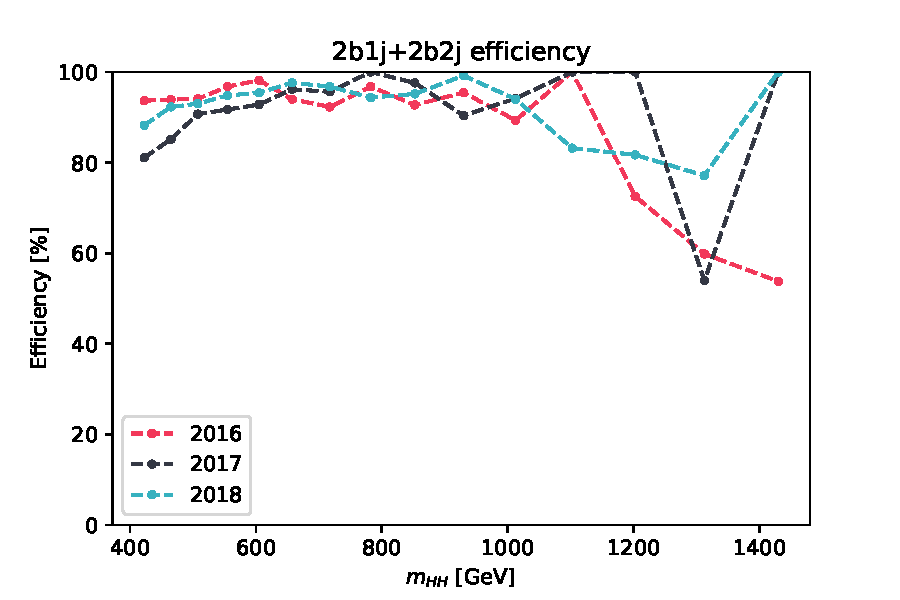
\includegraphics[width=0.33\textwidth]{\figpath/SMNR_VBF_502978-2b1j+2b2j-trigger-efficiency.pdf}
        }\\
        \caption{Trigger efficiencies of the 2b1j, 2b2j and combined for the MC16a/d/e corresponding to years 2016-2018 for various \HH signals as a function of \mhh.
        The bulk of the signal is around \SI{500}{\GeV}.
        A couple of bins in the high mass region are taking extreme values due to low statistics.
        Significantly lower efficiency for 2017 2b2j comparing to other years is due to tighter b-tagging requirement (lower efficiency).}
	\label{fig:HH_trigger_eff}
\end{figure}

\begin{figure}[htbp]
    \centering
    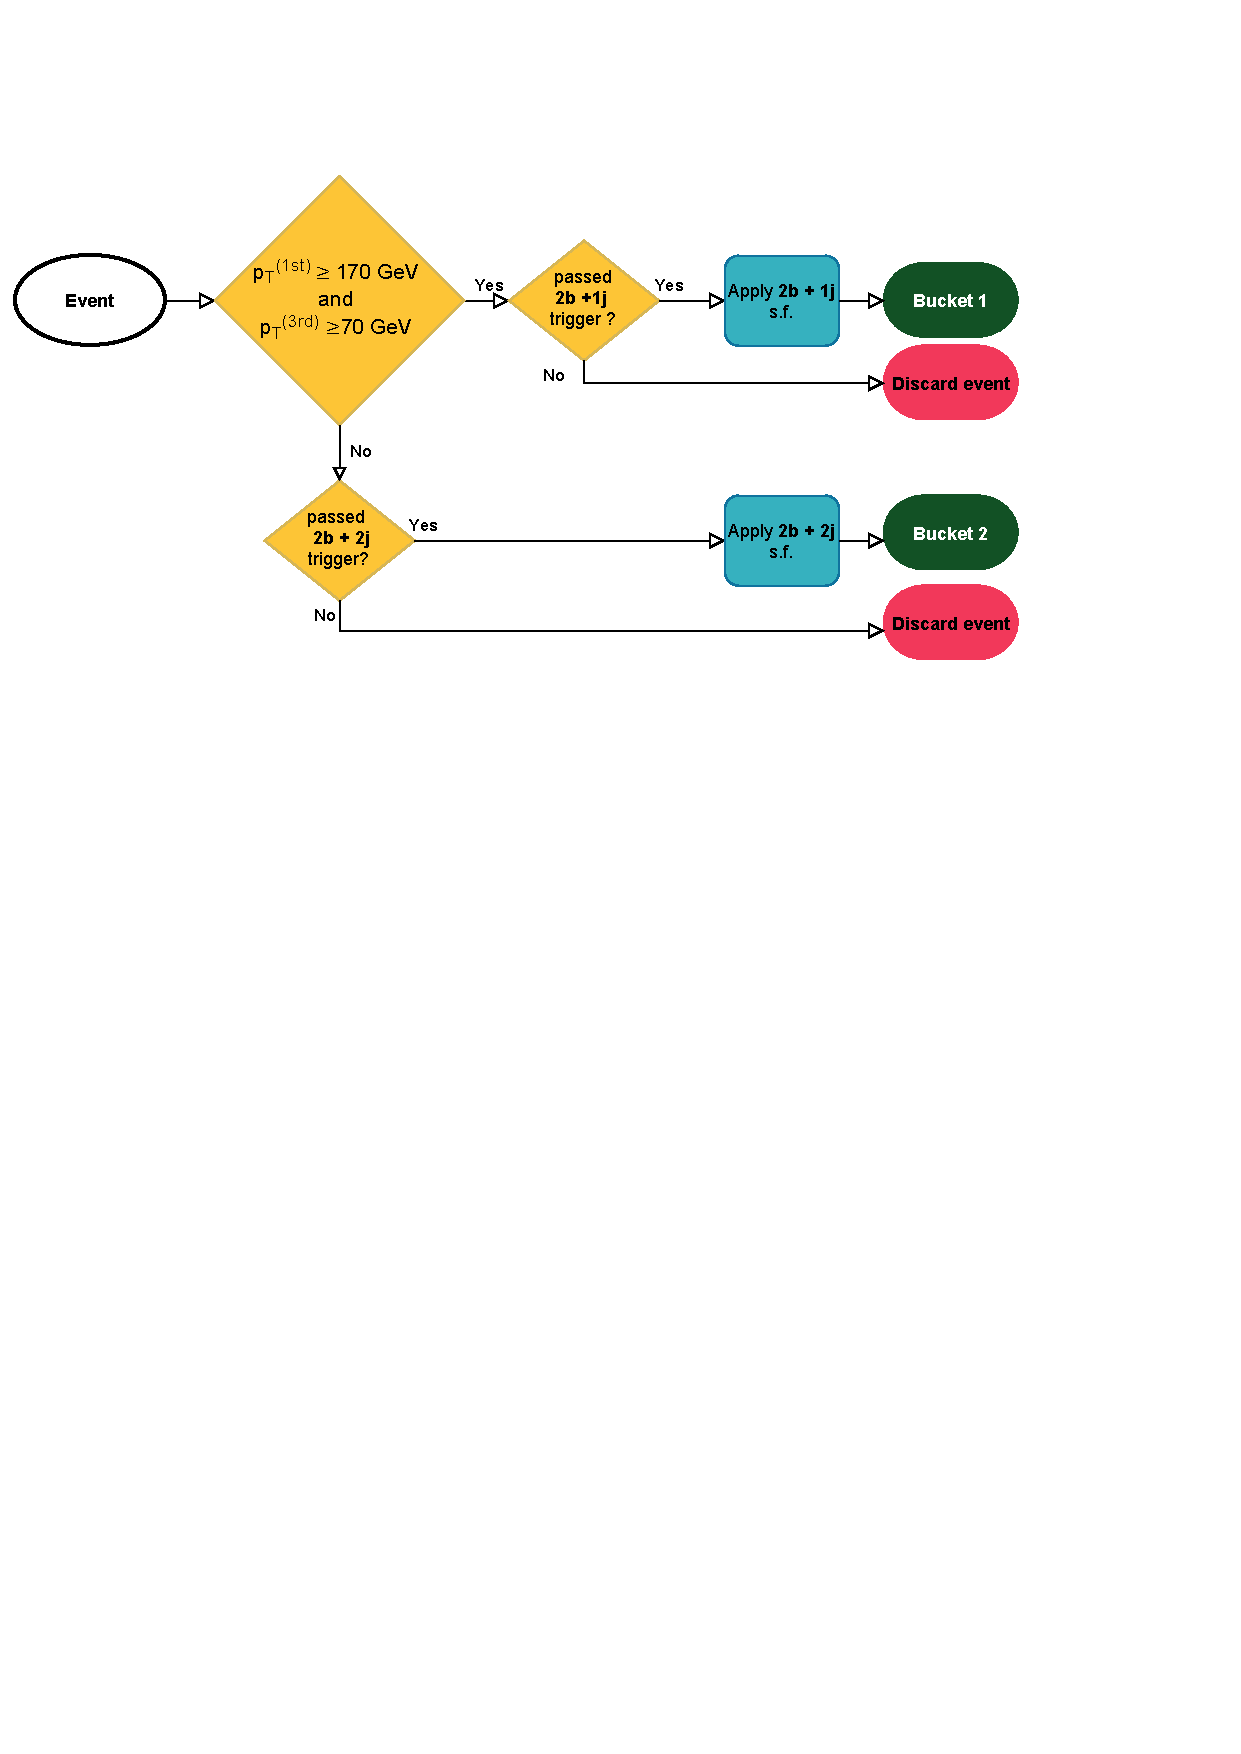
\includegraphics[width=0.8\textwidth]{\figpath/nr_buckets_diagram_simple.pdf}
    \caption{Trigger bucket strategy for non-resonant searches.}
    \label{fig:trigger-bucket-strategy}
\end{figure}


\hl{The details of the trigger names that we have are incredibly jargony, so I don't think I should include this table as is.}

\begin{table}[htbp]
\centering
\begin{tabular}{ccc}
Year                      & Trigger Name  & \textbf{Trigger Type}  \\ 
\hline
\multirow{2}{*}{2016}                      & HLT\_j100\_2j55\_bmv2c2060\_split                                               & 2b1j                   \\
                      & HLT\_2j35\_bmv2c2060\_split\_2j35\_L14J15.0ETA25                                & 2b2j                   \\

\hline

\multirow{2}{*}{2017}                      & HLT\_j110\_gsc150\_boffperf\_split\_2j35\_gsc55\_bmv2c1070\_split\_L1J85\_3J30  & 2b1j                   \\
                      & HLT\_2j15\_gsc35\_bmv2c1040\_split\_2j15\_gsc35\_boffperf\_split\_L14J15.0ETA25 & 2b2j                   \\

\hline

\multirow{2}{*}{2018}                      & HLT\_j110\_gsc150\_boffperf\_split\_2j45\_gsc55\_bmv2c1070\_split\_L1J85\_3J30  & 2b1j                   \\
                      & HLT\_2j35\_bmv2c1060\_split\_2j35\_L14J15.0ETA25                                & 2b2j                   \\
                
\end{tabular}
\caption{Triggers used for non-resonant searches.}
\label{tab:nr-triggers-used}
\end{table}

\begin{figure}
    \centering
    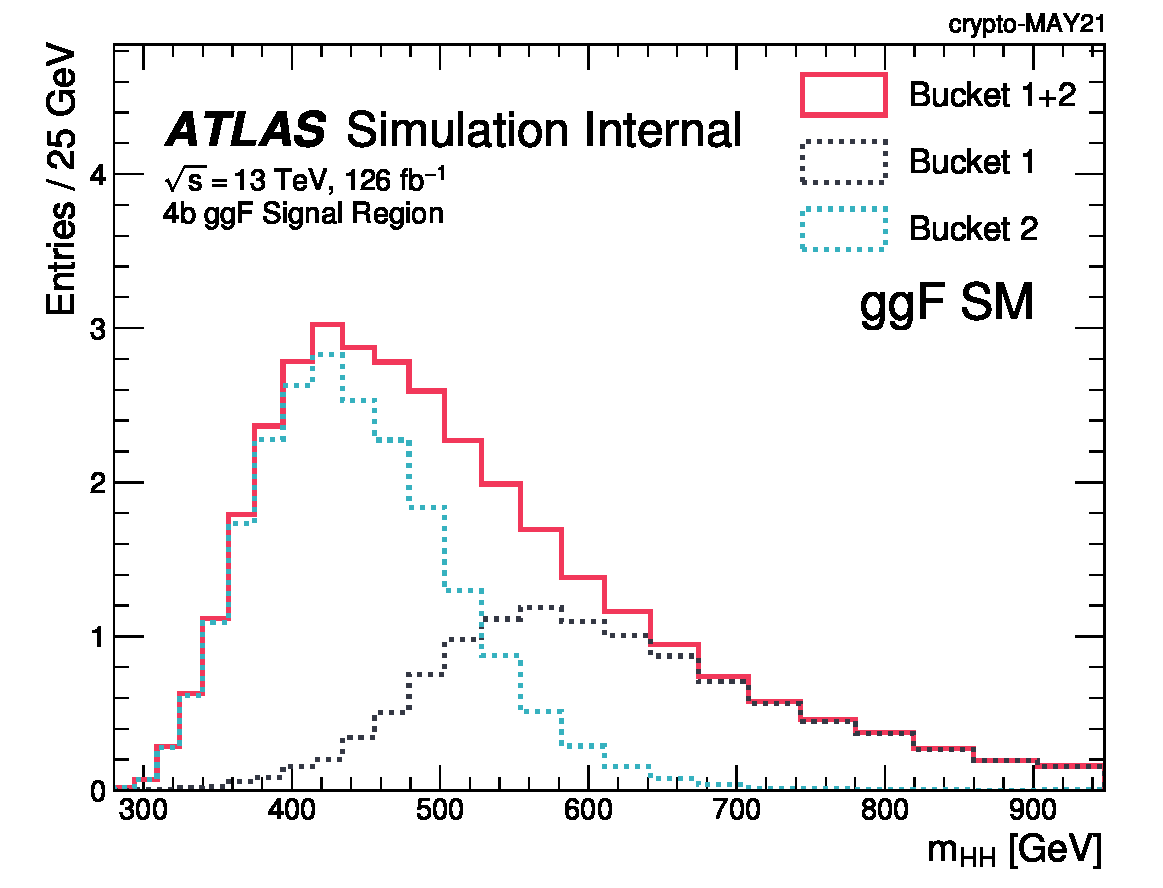
\includegraphics[width=0.48\textwidth]{\figpath/buckets_comparison_4b_ggF_SM_SR.pdf}
    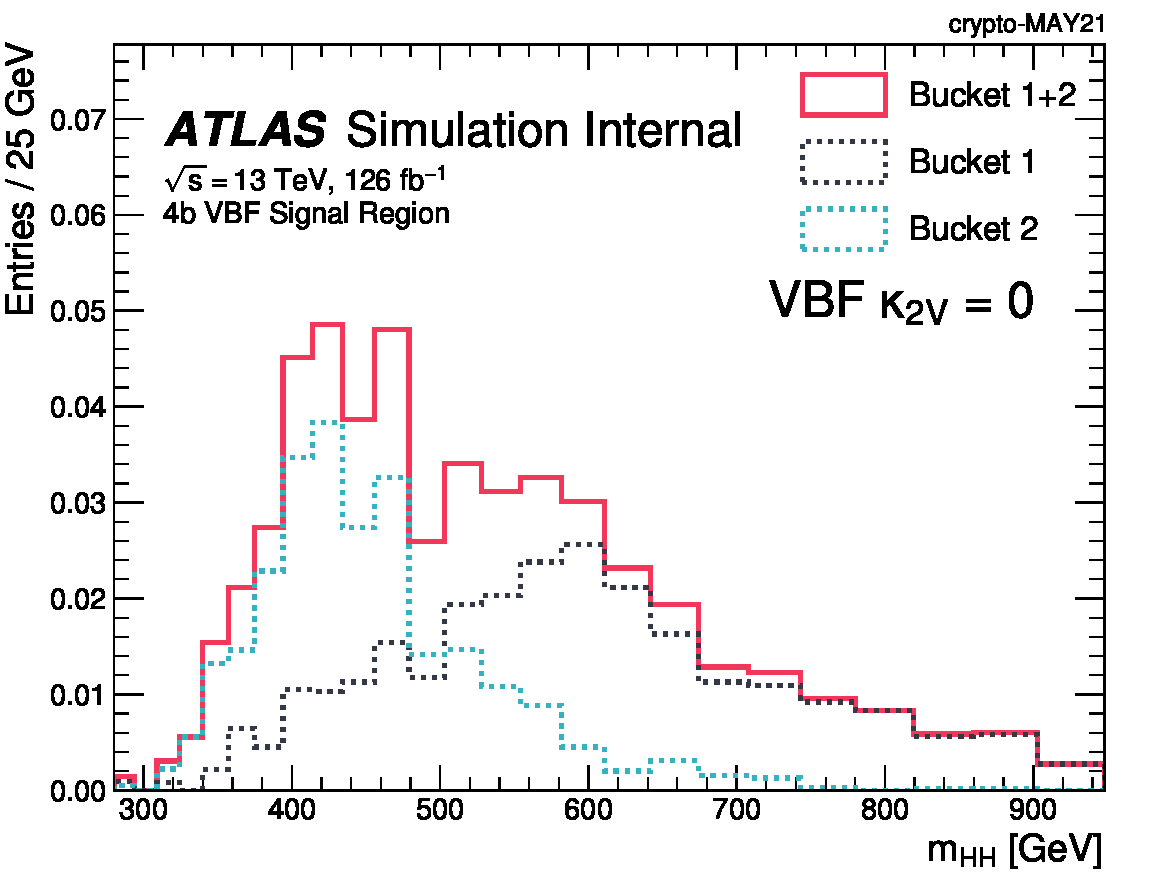
\includegraphics[width=0.48\textwidth]{\figpath/buckets_comparison_4b_VBF_SR.pdf}
    \caption{The bucket composition of \mhh for the SM ggF (left) and \kvv = 0 VBF (right) \HH MC simulation in the 4b Signal Regions.  Bucket 1 corresponds to the 2b1j trigger and Bucket 2 corresponds to the 2b2j trigger.}
    \label{fig:trig-bucket-4b}
\end{figure}


\begin{itemize}
   \item Type 1: A jet passes the online and offline \Pqb-tagging: 
	  \begin{equation}
		 \varepsilon(\text{on} \land \text{off}) 
		 = \varepsilon(\text{on} | \text{off}) \varepsilon(\text{off})
	  \end{equation}
   \item Type 2: A jet fails the online \Pqb-tagging and passes the offline \Pqb-tagging: 
	  \begin{equation}
		 \varepsilon(\overline{\text{on}} \land \text{off}) 
		 = [1 - \varepsilon(\text{on} | \text{off})] \varepsilon(\text{off})
	  \end{equation}
   \item Type 3: A jet passes the online \Pqb-tagging and fails the offline \Pqb-tagging: 
	  \begin{equation}\label{eq:sf-type3}
		 \varepsilon(\text{on} \land \overline{\text{off}}) 
		 = \varepsilon(\text{on}) - \varepsilon(\text{on} | \text{off}) \varepsilon(\text{off})
	  \end{equation}
   \item Type 4: A jet fails the online and offline \Pqb-tagging: 
	  \begin{equation}\label{eq:sf-type4}
		 \varepsilon(\overline{\text{on}} \land \overline{\text{off}}) 
		 = 1 - \varepsilon(\text{off}) - \varepsilon(\text{on}) + \varepsilon(\text{on} | \text{off}) \varepsilon(\text{off})
	  \end{equation}
\end{itemize}



\begin{figure}[ht]
    \centering
    \subfloat[1st jet at L1]{\label{fig:jet-level-trigSF17-2b1j-L1-1st}
            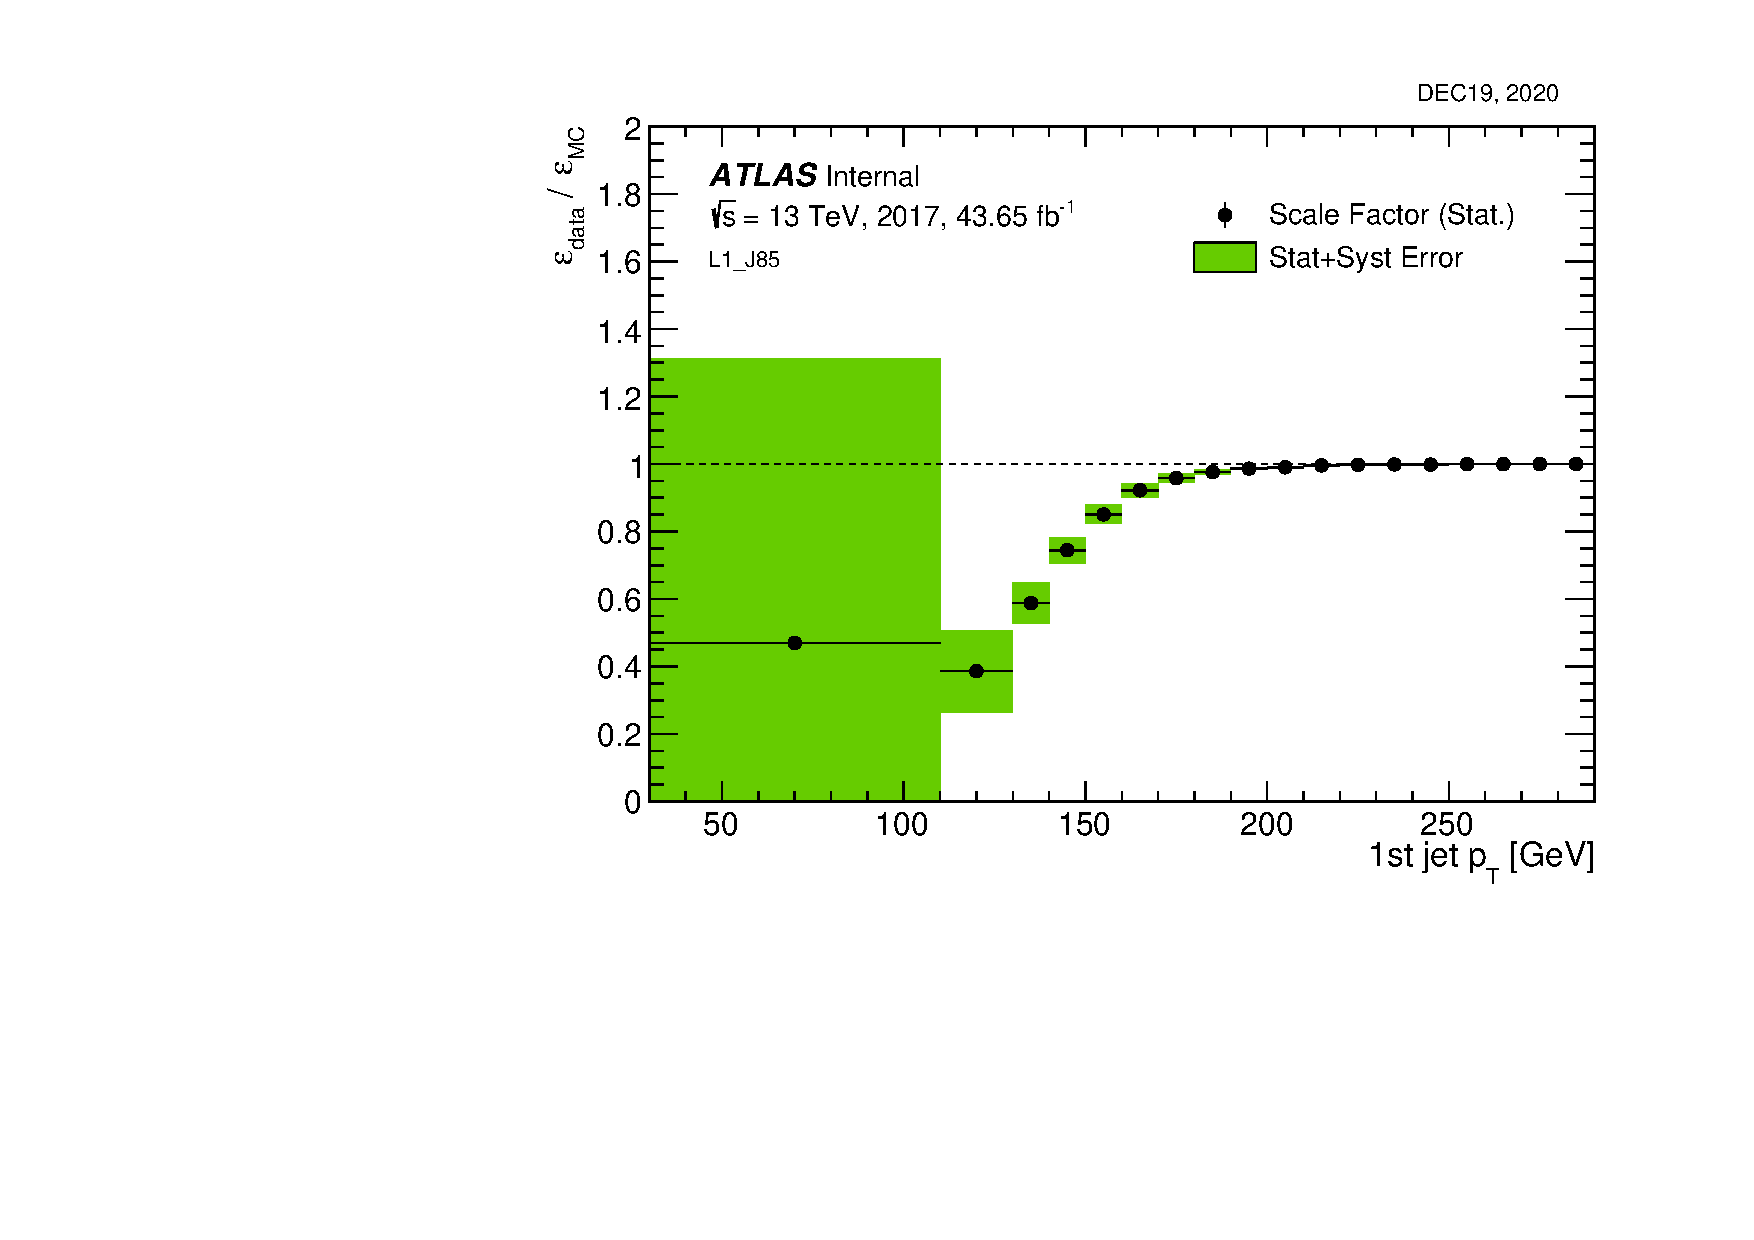
\includegraphics[width=0.3\textwidth]{figures/nr-int-note/appendices/jet-level-trigger-sf/V1/L1SF/2017/trigSF17-2b1j-L1-1st.pdf}
    }
    \subfloat[2nd jet at L1]{\label{fig:jet-level-trigSF17-2b1j-L1-2nd}
            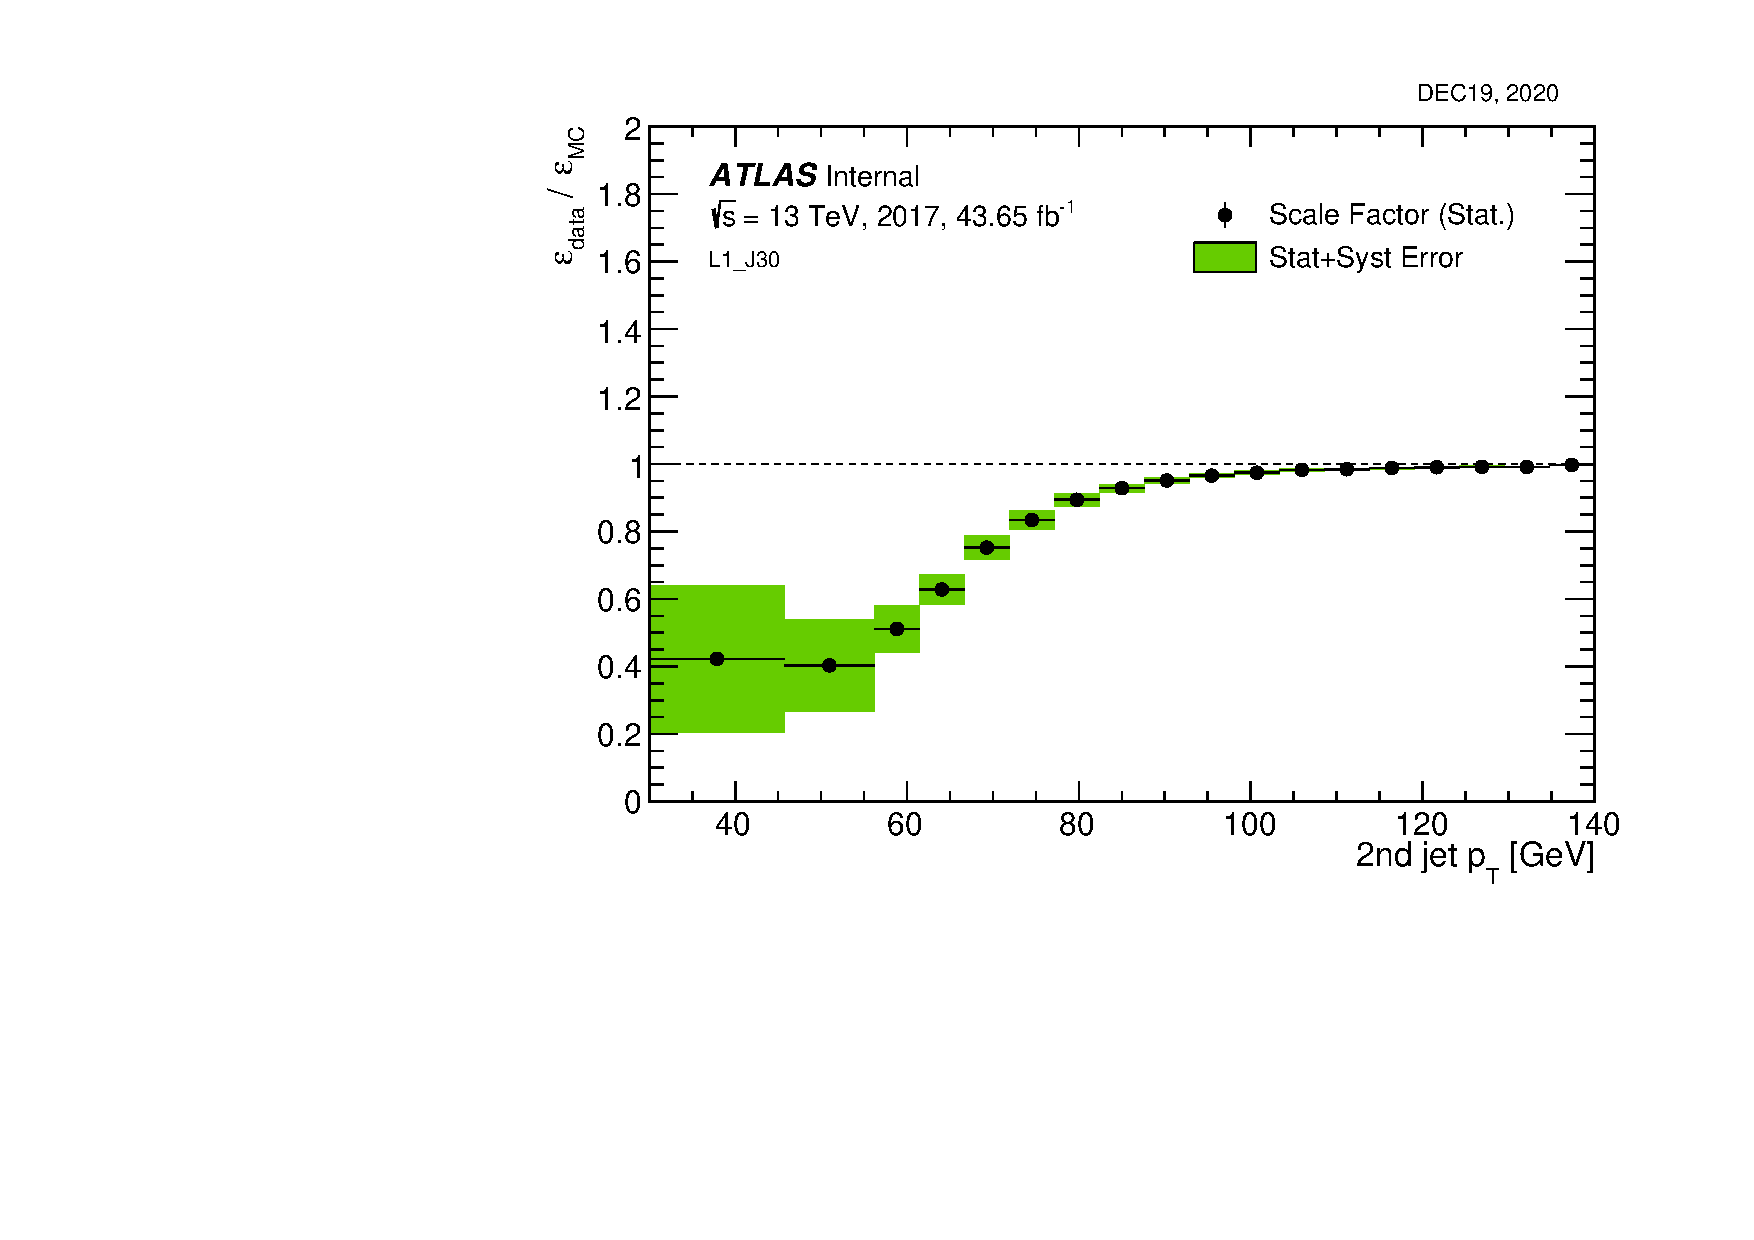
\includegraphics[width=0.3\textwidth]{figures/nr-int-note/appendices/jet-level-trigger-sf/V1/L1SF/2017/trigSF17-2b1j-L1-2nd.pdf}
    }
    \subfloat[3rd jet at L1]{\label{fig:jet-level-trigSF17-2b1j-L1-3rd}
            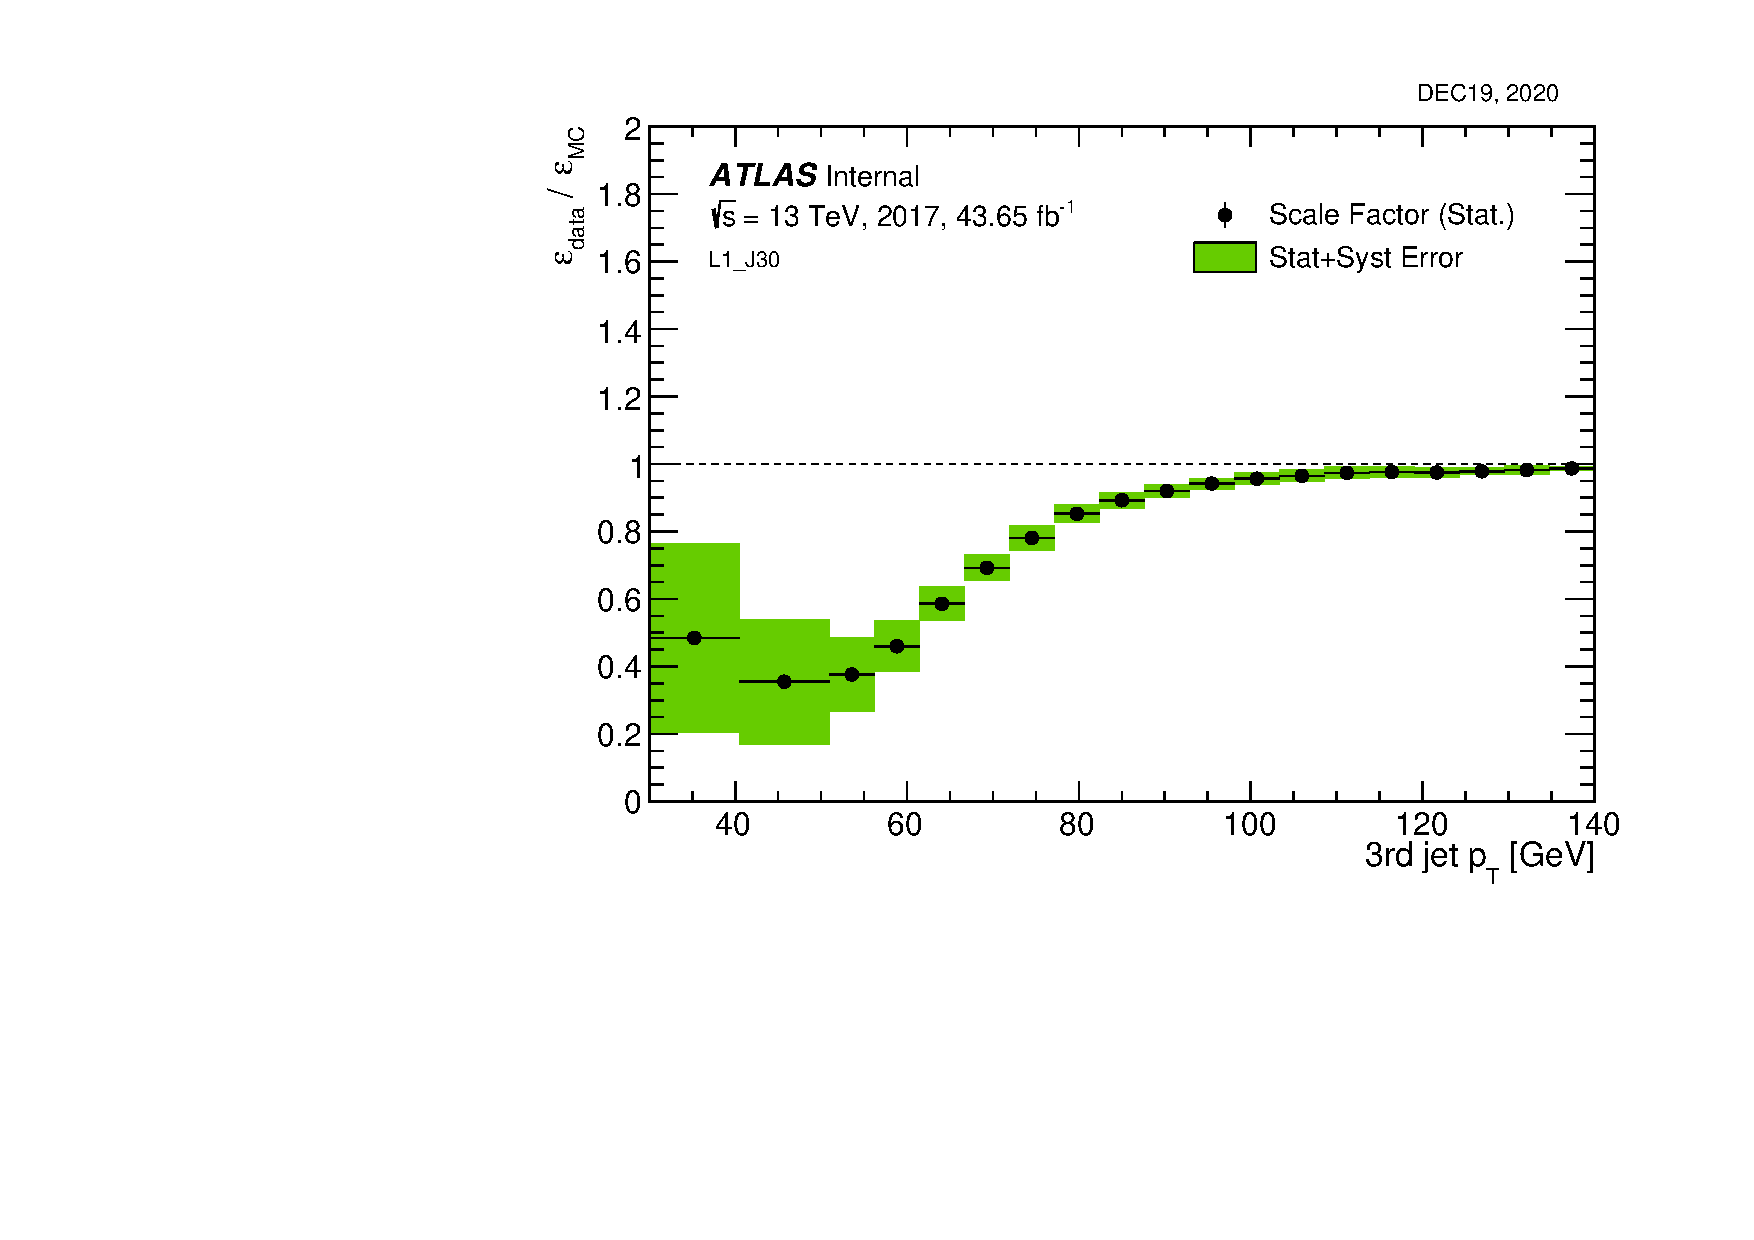
\includegraphics[width=0.3\textwidth]{figures/nr-int-note/appendices/jet-level-trigger-sf/V1/L1SF/2017/trigSF17-2b1j-L1-3rd.pdf}
    }

    \subfloat[1st jet at HLT]{\label{fig:jet-level-trigSF17-2b1j-HLT-1st}
            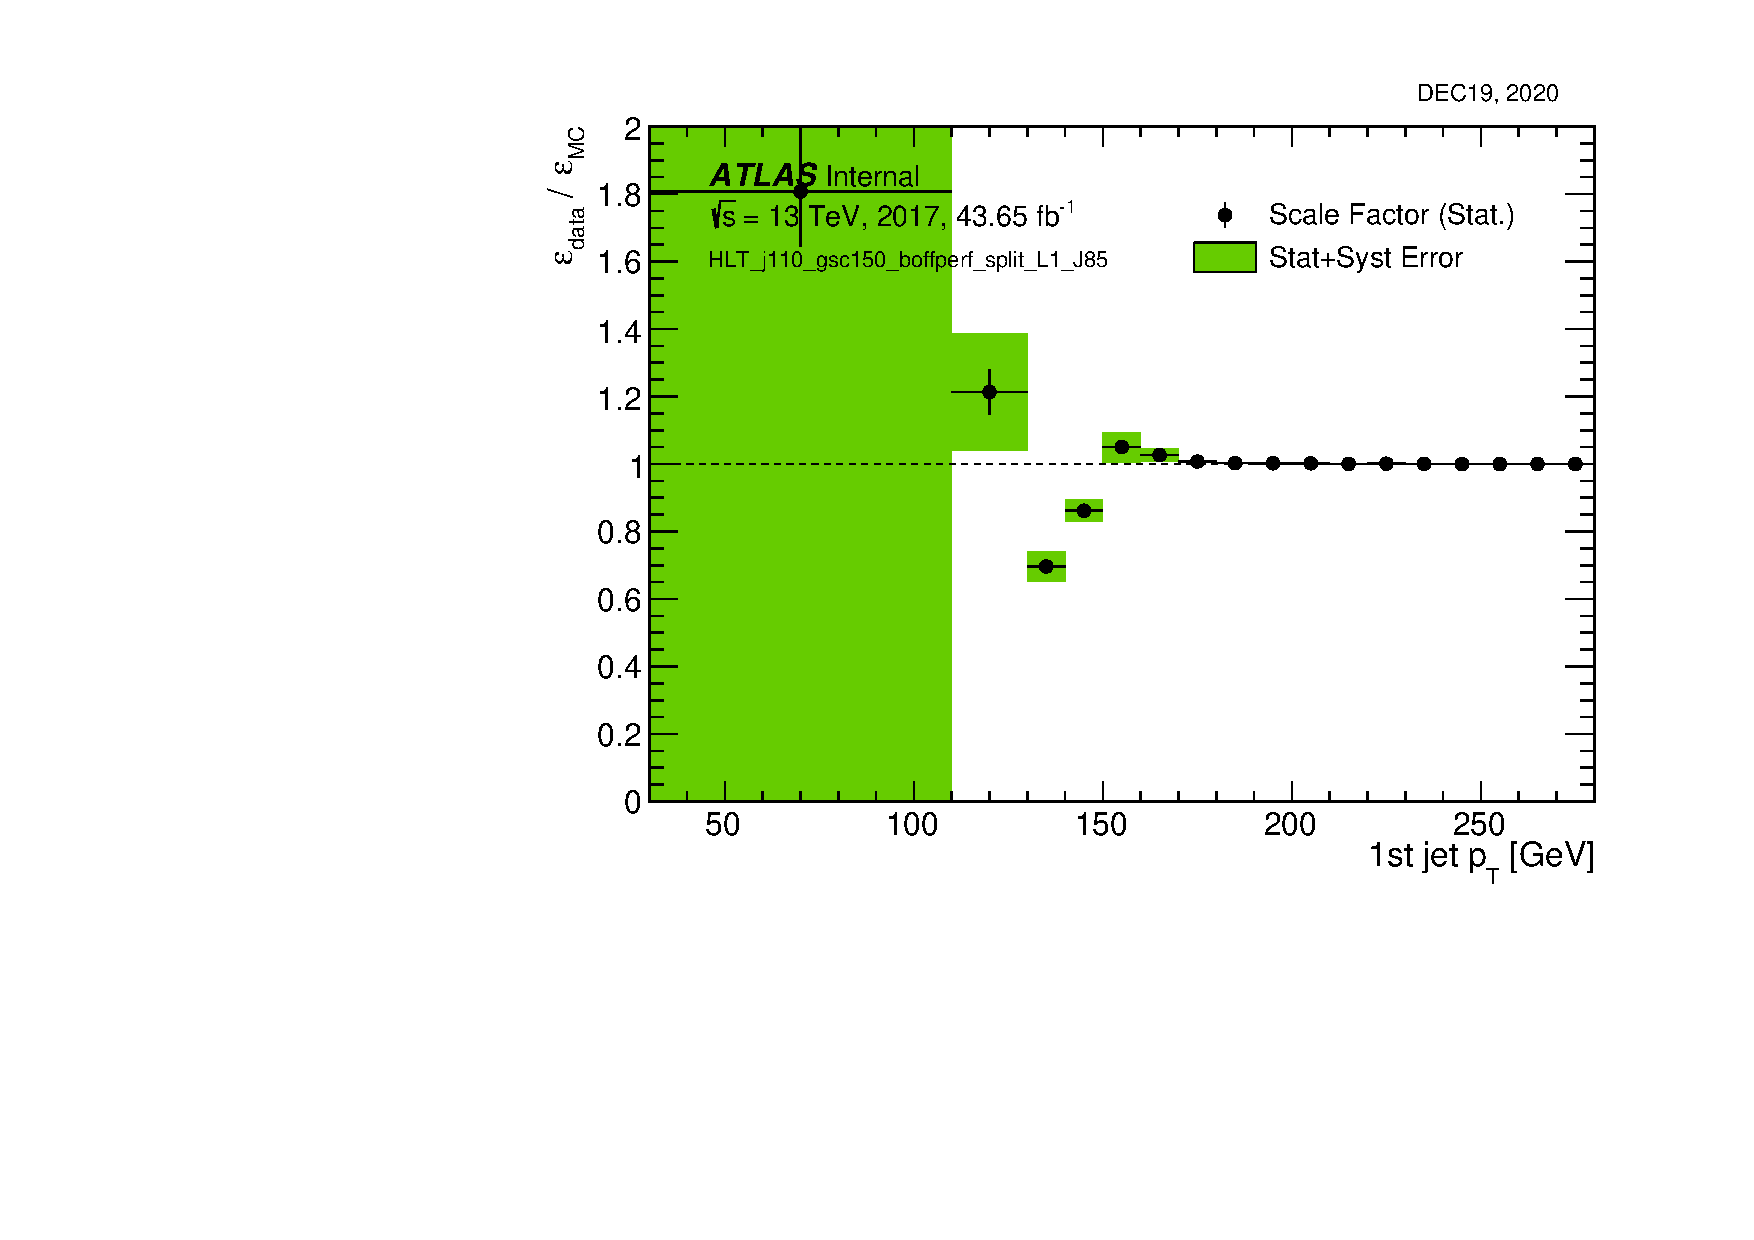
\includegraphics[width=0.3\textwidth]{figures/nr-int-note/appendices/jet-level-trigger-sf/V1/HLTSF/2017/trigSF17-2b1j-HLT-1st.pdf}
    }
    \subfloat[2nd jet at HLT]{\label{fig:jet-level-trigSF17-2b1j-HLT-2nd}
            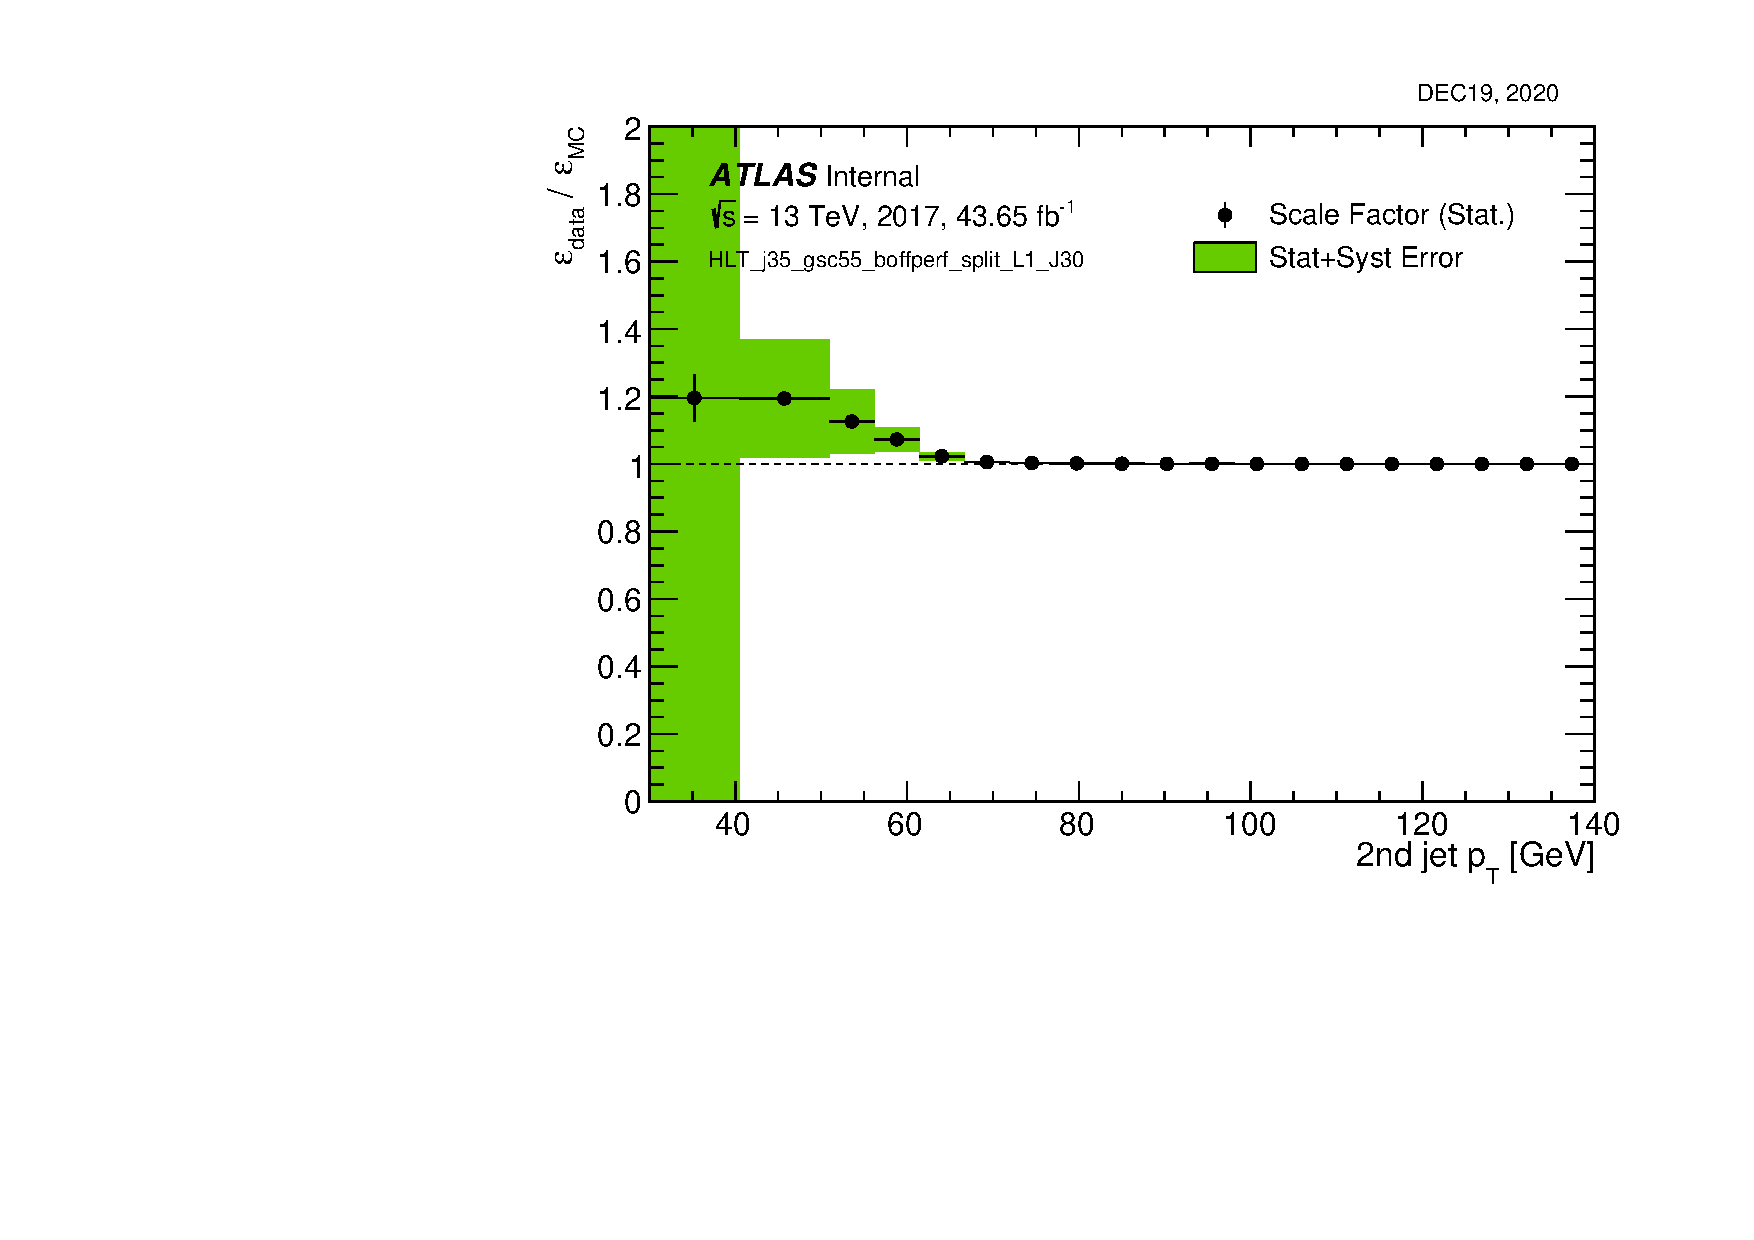
\includegraphics[width=0.3\textwidth]{figures/nr-int-note/appendices/jet-level-trigger-sf/V1/HLTSF/2017/trigSF17-2b1j-HLT-2nd.pdf}
    }
    \subfloat[3rd jet at HLT]{\label{fig:jet-level-trigSF17-2b1j-HLT-3rd}
            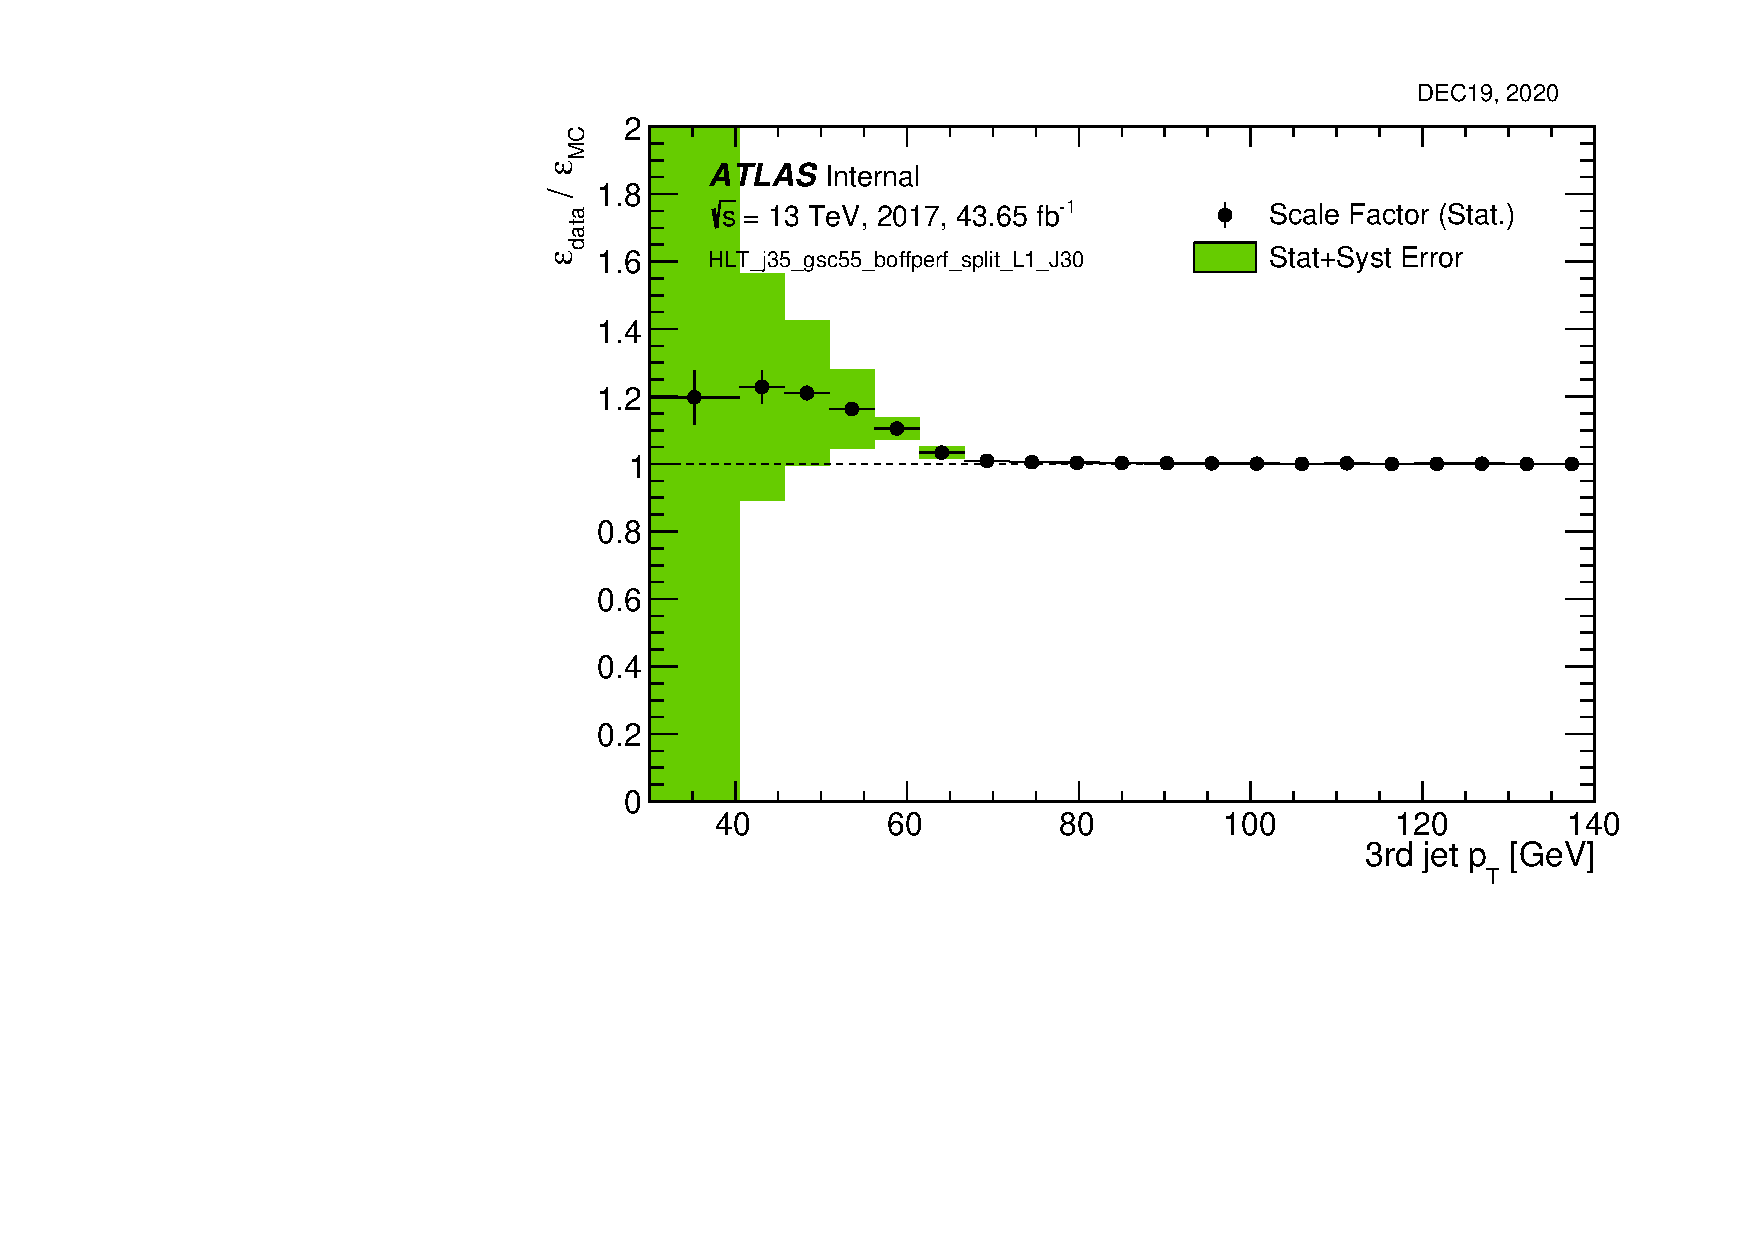
\includegraphics[width=0.3\textwidth]{figures/nr-int-note/appendices/jet-level-trigger-sf/V1/HLTSF/2017/trigSF17-2b1j-HLT-3rd.pdf}
    }

    \caption{Online jet kinematic scale factors of 2b1j trigger as a function of offline jet \pt in 2017. Vertical error bars include statistical uncertainties on the data, while the green bands correspond to the quadrature sum of statistical and systematic uncertainties.}
    \label{fig:jet-kinematict-trigSF17-2b1j}
\end{figure}
